%&custom12pt
%&LaTeX
\documentclass[titlepage,12pt,letterpaper]{article}\usepackage{float,amsmath,dcolumn,epsfig,ifthen,/Software/latex/vmargin,/Software/latex/harvard_mod}
%\pagestyle{empty}
%&custom12pt

\newcolumntype{d}[1]{D{.}{.}{#1}}
\setmarginsrb{1.2in}{1in}{1.2in}{1.4in}{0pt}{0pt}{0pt}{36pt}
% {left}{top}{right}{bottom}{headheight}{headsep}{footheight}{footskip}

%&custom12pt

\begin{document}

\begin{titlepage}

\hfill{\tiny EpidemiologySFI.tex}



\def\thefootnote{\fnsymbol{footnote}}

%\baselineskip=.2in

\enlargethispage{1000pt}
%\vspace{0.1in}

\centerline{\LARGE {The Epidemiology of Macroeconomic Expectations}}
\vspace{0.15in}

\centerline{\large Christopher D. Carroll$^{\dagger}$}
\centerline{ccarroll@jhu.edu}
\medskip
\medskip


%\vspace{0.1in}

\centerline{\today}

\vspace{0.1in}
\begin{table}[H]

%\vspace{.1in}
\centerline{\sc Abstract} 

Macroeconomists have long emphasized the importance of expectations in 
determining macroeconomic outcomes, and an enormous theoretical 
literature has developed examining many models of expectations 
formation.  This paper proposes a new approach, based on 
epidemiological models, in which only a small set of agents 
(professional forecasters) formulate their own expectations, which 
then spread through the population via the news media in a manner 
analogous to the spread of a disease.  The paper shows that the very 
simplest epidemiological model, called the `common source' model, does 
a good job of explaining the dynamics of inflation and unemployment 
expectations, and more complicated epidemiological models produce 
dynamics similar to those that emerge from the common source model.

\medskip \medskip {\bf Keywords}: inflation, expectations, unemployment,
monetary policy, agent-based modeling

\medskip
\medskip
{\bf JEL Classification Codes: D84, E31} 

\medskip
\medskip

This paper was written in connection with the conference ``The Economy 
As an Evolving Complex System III'' at the Santa Fe Institute in 
November of 2001, in honor of Kenneth Arrow's contributions to the 
Santa Fe Institute and to economics.  A companion paper, 
``Macroeconomic Expectations of Households and Professional 
Forecasters,'' presents empirical work that was part of an earlier 
draft of this paper; that paper was published in the {\it Quarterly 
Journal of Economics}, Vol. 118, Number 1 (February 2003), pp. 269--298.

\medskip

{\small 
\input titlepage_thanks.tex
}

\medskip\medskip

{\small The data, econometric programs, and simulation programs that generated 
all of the results in this paper are available on the author's 
website, http://www.econ.jhu.edu/people/carroll.

\medskip\medskip\medskip

$^{\dagger}$  Department of Economics, Johns Hopkins University, Baltimore MD 21218-2685.
}
\end{table}

\clearpage\pagebreak\vfill\eject

\end{titlepage}

\sloppy 
%\renewcommand{\hbadness}{10000}

\section{Introduction}

\thispagestyle{empty}
%\large \setmarginsrb{0.8in}{0.5in}{0.5in}{0.5in}{0pt}{0pt}{0pt}{0pt}% {left}{top}{right}{bottom}{headheight}{headsep}{footheight}{footskip}\pagestyle{empty}

Economists have long understood that macroeconomic outcomes depend
critically upon agents' expectations.
Keynes~\cite{keynes:generaltheory} believed that economies could
experience booms and busts that reflected movements in `animal
spirits' (a view that has some appeal at the current moment of dot-com
hangover), but the basis for most of today's macro models is the
rational expectations approach pioneered in the 1970s by Lucas,
Sargent, Barro, and others.  This approach makes a set of assumptions
that are much stronger than rationality alone.  In particular, the
framework assumes that all agents in the economy are not merely
rational, but also share identical (correct) beliefs about the
structure of the economy, and have instantaneous and costless access
to all the latest economic data.  Each agent combines these data with
the true macroeconomic model to obtain a forecast for the future path
of the economy, on the assumption that all other agents have identical
beliefs and information (and therefore forecasts).

This set of assumptions has turned out to be a powerful vehicle for
macroeconomic modeling, but has never been free from the criticism
that it does not resemble the real world of conflicting opinions and
forecasts, workers (and even some business leaders) who may not pay
much attention to macroeconomic matters, and information that can
sometimes be costly to obtain and process.  Rational expectations
models also have problems explaining some robust stylized facts, such
as the apparent inexorability of the tradeoff between inflation and
unemployment rate (see Ball~\cite{ball:sacrifice} or
Mankiw~\cite{mankiw:inexorable}).  Partly in response to these
problems, an emerging literature has been exploring models based on an
assumption that agents engage in some form of data-based learning
process to form their expectations; for surveys, see
Sargent~\cite{sargent:bounded} or Evans and
Honkapohja~\cite{evans&honk:book}.  But the rational expectations
framework remains the dominant approach, partly because it tends to be
mathematically more tractable than many proposed alternatives.

This paper proposes a tractable alternative framework for the 
formation of a typical person's expectations.  Rather than having 
their own macroeconomic model and constantly feeding it the latest 
statistics, typical people are assumed to obtain their views about the 
future path of the economy from the news media, directly or 
indirectly.  Furthermore (and importantly), not every person pays 
close attention to all macroeconomic news; instead, people are assumed 
to absorb the economic content of news reports probabilistically, in a
way that resembles the spread of disease in a population, so 
that it may take quite some time for news of changed macroeconomic 
circumstances to penetrate to all agents in the economy.  

Roberts~\cite{roberts:inflexp} and Mankiw and
Reis~\cite{mankiw&reis:slumps,mankiw&reis:stickye} have recently
proposed aggregate expectations equations that are mathematically very
similar to aggregate implications of the baseline epidemiological
model of expectations proposed derived here.  Roberts's work was
motivated by his separate findings in
Roberts~\cite{roberts:phillips,roberts:stickyinfl} that empirical
macro models perform better in a variety of dimensions when
survey-based inflation expectations are used in place of constructed
model-consistent rational expectations.  Mankiw and
Reis~\cite{mankiw&reis:slumps,mankiw&reis:stickye} obtain similar
findings, and particularly emphasize the point that these models can
explain the inexorability of an inflation-unemployment tradeoff much
better than the standard model with rational expectations does.

However, neither Roberts~\cite{roberts:inflexp} nor Mankiw and
Reis~\cite{mankiw&reis:slumps,mankiw&reis:stickye} devote much effort
to explaining {\it why} the dynamics of aggregate expectations should
evolve as they proposed (though Roberts does suggest that his equation
might result from the diffusion of press reports).  Mankiw and Reis
motivate their model by suggesting that there are costs either of
obtaining or of processing inflation every time an agent updates;
however, they do not provide an explicit information-costs or
processing-costs microfoundation.

This paper provides an explicit microfoundation for a simple aggregate
expectations equation, based on simple models of the spread of
disease.  Rather than tracking the spread of a disease through a
population, the model tracks the spread of a piece of information
(specifically, the latest rational forecast of inflation).

A companion paper, Carroll~\cite{carroll:epidemicinflQJE}, estimates 
the baseline model and finds that it does a good job at capturing the 
dynamics of household survey expectations about both inflation and 
unemployment.  Furthermore, that paper shows that household inflation 
expectations are closer to the expectations of professional 
forecasters during periods when there is more news coverage of 
inflation, and that the speed with which household expectations adjust 
to professional expectations is faster when there is more news 
coverage.

After providing the epidemiological foundation for the model estimated
in Carroll~\cite{carroll:epidemicinflQJE} and summarizing the basic
empirical results from that paper, this paper explores the
implications of several extensions to the model, using the kinds of
`agent-based' simulation techniques pioneered at the Santa Fe
Institute and at the Center for Social and Economic Dynamics (CSED) at
the Brookings Institution.

The first extension is to allow heterogeneity in the extent to which 
different households pay attention to macroeconomic news.  This 
version of the model is capable of generating demographic differences 
in macroeconomic expectations like those documented in 
Souleles~\cite{souleles:sentiment}, which are very hard to rationalize 
in a rational expectations model.  Both this extension and the 
baseline version of the model are then simulated in order to derive 
implications for the standard deviation of inflation expectations 
across agents.  When the simulated data are compared to the empirical 
data, the results are mixed.  On one hand, the patterns over time of 
the empirical and the simulated standard deviations bear a strong 
resemblance, rising sharply in the late 1970s and early 1980s and then 
gradually falling off again.  On the other hand, the {\it level} of 
the standard deviation in the empirical data is much higher than in 
the simulated data; however, I show that adding simple forms of memory 
error can make the model and the data match up reasonably well.

The next extension examines what happens when the model is generalized 
to a more standard epidemiological context: A `random mixing' 
framework in which people can be `infected' with updated inflation 
expectations by conversations with random other individuals in the 
population.  It turns out that when the baseline framework that 
assumes infection only from news sources is estimated on simulated 
data from the random mixing model, the baseline framework does an 
excellent job of capturing the dynamics of mean inflation 
expectations; this suggests that the `common source' simplification is 
probably not too problematic.

The final extension is to a context in which people communicate only 
with near `neighbors' in some social sense, rather than with random 
other individuals in the population.  Simulation and estimation of the 
baseline model on this population finds that the baseline model again 
does a good job of capturing expectational dynamics; however, in one 
particular respect the results in this framework are a better match 
for the empirical results than is the baseline model.

The paper concludes with some general lessons and ideas for future 
research.

\section{The Epidemiology of Expectations}

% Brief treatment of classical disease in well-mixed population

\subsection{The SIR Model}
Epidemiologists have developed a rich set of models for the 
transmission of disease in a population.  The general framework 
consists of a set of assumptions about who is susceptible to the 
disease, who among the susceptible becomes infected, and whether and 
how individuals recover from the infection (leading to the framework's 
designation as the `SIR' model).

The standard assumption is that a susceptible individual who is exposed 
to the disease in a given period has a fixed probability $p$ of 
catching the disease.  Designating the set of newly infected 
individuals in period $t$ as $N_{t}$ and the set of susceptible 
individuals as $S_{t}$,
\begin{eqnarray}
        N_{t} & = & p S_{t}.
\end{eqnarray}

The next step is to determine susceptibility.  The usual assumption is 
that in order to be susceptible, a healthy individual must have 
contact with an already-infected person.  In a population where each 
individual has an equal probability of encountering any other person 
in the population (a `well-mixed' population), the growth rate of the 
disease will depend upon the fraction of the population already 
infected; if very few individuals are currently infected, the small 
population of diseased people can infect only a small absolute number 
of new victims.

However, there is a special case that is even simpler.  This occurs 
when the disease is not spread person-to-person, but through contact 
with a `common source' of infection.  The classic example is 
Legionnaire's disease, which was transmitted to a group of hotel 
guests via a contaminated air conditioning system (see Fraser et.  
al.~\cite{medline:legionnaires} for a description from the 
epidemiological literature).  Another application is to illness caused 
by common exposure to an environmental factor such as air pollution.  
In these cases, the transmission model is extremely simple: Any 
healthy individual is simply assumed to have a constant probability 
per period of becoming infected from the common source.  This is the 
case we will examine, since below we will assume that news reports 
represent a `common source' of information available to all members of 
the population.

One further assumption is needed to complete the model: The 
probability that someone who is infected will recover from the 
disease.  The simplest possible assumption (which we will use) is that 
infected individuals never recover.

Under this set of assumptions, the dynamics of the disease are as 
follows.  In the first period, proportion $p$ of the population 
catches the disease, leaving $(1-p)$ uninfected.  In period 2, 
proportion $p$ of these people catch the disease, leading to a new 
infection rate of $p(1-p)$ and to a fraction $p+p(1-p)$ of the 
population being infected.  Spinning this process out, it is easy to 
see that starting from period 0 at the beginning of which nobody is 
infected, the total proportion infected at the end of $t$ periods is
\begin{eqnarray}
        \mbox{Fraction Ill} & = & p+p(1-p)+p(1-p)^{2} \ldots + p(1-p)^{t} \label{eq:diseasep} \\
         & = & p \sum_{s=0}^{t} (1-p)^{s} 
\end{eqnarray}
whose limit as $t \rightarrow \infty$ is $p/p=1$, implying that (since 
there is no recovery) everyone will eventually become infected.  In 
the case where `infection' is interpreted as reflecting an agent's 
knowledge of a piece of information, this simply says that eventually 
everyone in the economy will learn a given piece of news.

\subsection{The Epidemiology of Inflation Expectations}

Now consider a world where most people form their expectations about
future inflation by reading newspaper articles.  Imagine for the
moment that every newspaper inflation article contains a complete
forecast of the inflation rate for all future quarters, and suppose
(again momentarily) that any person who reads such an article can
subsequently recall the entire forecast.  Finally, suppose that at any
point in time $t$ all newspaper articles print identical
forecasts.\footnote{This subsection is largely drawn from
Carroll~\cite{carroll:epidemicinflQJE}; however, that paper does not
discuss the epidemiological interpretation of the derivations, as this
derivation does.}

Assume that not everybody reads every newspaper article on inflation.  
Instead, reading an article on inflation is like becoming infected 
with a common-source disease: In any given period each individual 
faces a constant probability $\lambda$ of becoming `infected' with the 
latest forecast by reading an article.  Individuals who do not 
encounter an inflation article simply continue to believe the last 
forecast they read about.\footnote{This is mathematically very similar 
to the Calvo~\cite{calvoPrices} model in which firms change their 
prices with probability $p$.}

Call $\pi_{t+1}$ the inflation rate between quarter $t$ and quarter $t+1$,
\begin{eqnarray}
        \pi_{t+1} & = & \log(p_{t+1})-\log(p_{t}),
\end{eqnarray}
where $p_{t}$ is the aggregate price index in period $t$.  If we 
define $M_{t}$ as the operator that yields the population-mean value 
of inflation expectations at time $t$ and denote the {\bf N}ewspaper 
forecast printed in quarter $t$ for inflation in quarter $s \geq t$ as 
$N_{t}[\pi_{s}]$, by analogy with equation~\eqref{eq:diseasep} we have 
that
\begin{eqnarray}
        M_{t}[\pi_{t+1}] & = & \lambda N_{t}[\pi_{t+1}]
        +(1-\lambda) \left\{ \lambda N_{t-1}[\pi_{t+1}]
        +(1-\lambda)\left(\lambda N_{t-2}[\pi_{t+1}] 
        + \ldots\right) \right\} \nonumber \\ \label{eq:stickyerat}
\end{eqnarray}

The derivation of this equation is as follows.  In period $t$ a 
fraction $\lambda$ of the population will have been `infected' with 
the current-period newspaper forecast of the inflation rate next 
quarter, $N_{t}[\pi_{t+1}]$.  Fraction $(1-\lambda)$ of the population 
retains the views that they held in period $t-1$ of period $t+1$'s 
inflation rate.  Those period-$t-1$ views in turn can be decomposed 
into a fraction $\lambda$ of people who encountered an article in 
period $t-1$ and obtained the newspaper forecast of period $t+1$'s 
forecast, $N_{t-1}[\pi_{t+1}]$, and a fraction $(1-\lambda)$ who 
retained their period-$t-2$ views about the inflation forecast in 
period $t+1$.  Recursion leads to the remainder of the equation.

This expression for inflation expectations is identical to the one
proposed by Mankiw and
Reis~\cite{mankiw&reis:slumps,mankiw&reis:stickye}, except that in
their model the updating agents construct their own rational forecast
of the future course of the macroeconomy rather than learning about
the experts' forecast from the news media.  The equation is also
similar to a formulation estimated by
Roberts~\cite{roberts:stickyinfl}, except that Roberts uses past
realizations of the inflation rate on the right hand side rather than
past forecasts.

Mankiw and Reis loosely motivate the equation by arguing that
developing a full-blown inflation forecast is a costly activity, which
people might therefore engage in only occasionally.  It is undoubtedly
true that developing a reasonably rational quarter-by-quarter forecast
of the inflation rate arbitrarily far into the future would be a very
costly enterprise for a typical person.  If this were really what
people were doing, one might expect them to make forecasts only very
rarely indeed.  However, reading a newspaper article about inflation,
or hearing a news story on television or the radio, is not costly in
either time or money.  There is no reason to suppose that people need
to make forecasts themselves if news reports provide such forecasts
essentially for free.  Thus the epidemiological derivation of this
equation seems considerably more attractive than the loose
calculation-costs motivation provided by Mankiw and Reis, both because
this is a fully specified model and because it delivers further
testable implications (for example, if there is empirical evidence
that people with higher levels of education are more likely to pay
attention to news, the model implies that their inflation forecasts
will on average be closer to the rational forecast; see below for more
discussion of possible variation in $\lambda$ across population
groups).

Of course, real newspaper articles do not contain a quarter-by-quarter 
forecast of the inflation rate into the infinite future as assumed in 
the derivation of \eqref{eq:stickyerat}, and even if they did it is 
very unlikely that a typical person would be able to remember the 
detailed pattern of inflation rates far into the future.  In order
to relax these unrealistic assumptions it turns out to be necessary 
to impose some structure on households' implicit views about the
inflation process.

Suppose people believe that at any given time the economy has an 
underlying ``fundamental'' inflation rate.  Furthermore, suppose 
people believe that future changes in the fundamental rate are 
unforecastable; that is, after the next period the fundamental rate 
follows a random walk.  Finally, suppose the person believes that 
the actual inflation rate in a given quarter is equal to that period's 
fundamental rate plus an error term $\epsilon_{t}$ which reflects 
unforecastable transitory inflation shocks (reflected in the `special 
factors' that newspaper inflation stories often emphasize).  Thus, the 
person believes that the inflation process is captured by
\begin{eqnarray}
        \pi_{t} & = & \pi_{t}^{f}+\epsilon_{t}            \label{eq:Fpi} 
\\   \pi_{t+1}^{f} & = & \pi_{t}^{f}+\eta_{t+1}  \label{eq:Fpi2},
%\\   \pi_{t+2}^{f} & = & \pi_{t+1}^{f}+\eta_{t+2}  \label{eq:Fpi3}
\\ \phantom{456}\vdots\phantom{3} & & 
\phantom{\ldots .}\vdots\phantom{\ldots} \nonumber
\end{eqnarray}
where $\epsilon_{t}$ is a transitory shock to the inflation rate in 
period $t$ while $\eta_{t}$ is the permanent innovation in the 
fundamental inflation rate in period $t$.  We further assume that 
consumers believe that values of $\eta$ beyond period $t+1$, and 
values of $\epsilon$ beyond period $t$, are unforecastable white noise 
variables; that is, future changes in the fundamental inflation rate 
are unforecastable, and transitory shocks are expected to go 
away.\footnote{Note that we are allowing people to have some idea 
about how next quarter's fundamental rate may differ from the current 
quarter's rate, because we did not impose that consumers' expectations 
of $\eta_{t+1}$ must equal zero.}

Before proceeding it is worth considering whether this is a plausible 
view of the inflation process; we would not want to build a model on 
an assumption that people believe something patently absurd.  
Certainly, it would not be plausible to suppose that people always and 
everywhere believe that the inflation rate is characterized 
by~\eqref{eq:Fpi}-\eqref{eq:Fpi2}; for example, 
Ball~\cite{ball:nearrational} shows that in the US from 1879-1914 the 
inflation rate was not persistent in the US, while in other countries 
there have been episodes of hyperinflation (and rapid disinflation) in 
which views like~\eqref{eq:Fpi}-\eqref{eq:Fpi2} would have been 
nonsense.

However, the relevant question for the purposes of this paper is 
whether this view of the inflation process is plausible for the period 
for which I have inflation expectations data.  Perhaps the best way to 
examine this is to ask whether the univariate statistical process for 
the inflation rate implied by \eqref{eq:Fpi} and \eqref{eq:Fpi2} is 
strongly at odds with the actual univariate inflation process.  In 
other words, after allowing for transitory shocks, does the inflation 
rate approximately follow a random walk?

\input DataAndPrograms/Volumes/Data/ADFpi.tex

The appropriate statistical test is an augmented Dickey-Fuller test.  
Table~\ref{table:ADFpi} presents the results from such a test.  The 
second row shows that even with more than 160 quarters of data it is 
not possible to reject at a 5 percent significance level the 
proposition that the core inflation rate follows a random walk with a 
one-period transitory component - that is, it is not possible to 
reject the process defined 
by~\eqref{eq:Fpi}-\eqref{eq:Fpi2}.\footnote{The near-unit-root feature 
of the inflation rate in the post-1959 period is well known to 
inflation researchers; some authors find that a unit root can be 
rejected for some measures of inflation over some time periods, but it 
seems fair to say that the conventional wisdom is that at least since 
the late 1950s inflation is `close' to a unit root process.  See 
Barsky~\cite{barsky:fisher} for a more complete analysis, or 
Ball~\cite{ball:nearrational} for a more recent treatment.} When the 
transitory shock is allowed to have effects that last for two quarters 
rather than one, it is not possible to reject a random walk in the 
fundamental component even at the 10 percent level of significance 
(the last row in the table).

Note that the unit root (or near unit root) in inflation does not 
imply that future inflation rates are totally unpredictable, only that 
the history of inflation by itself is not very useful in forecasting 
future inflation {\it changes} (beyond the disappearance of the 
transitory component of the current period's shock).  This does not 
exclude the possibility that current and lagged values of other 
variables might have predictive power.  Thus, this view of the 
inflation rate is not necessarily in conflict with the vast and 
venerable literature showing that other variables (most notably the 
unemployment rate) do have considerable predictive power for the 
inflation rate (see Staiger, Stock, and Watson~\cite{ssw:nairu} for a 
recent treatment).

Suppose now that rather than containing a forecast for the entire 
quarter-by-quarter future history of the inflation rate, newspaper 
articles simply contain a forecast of the inflation rate over the next 
year.  The next step is to figure out how such a one-year forecast for 
inflation can be integrated into some modified version of 
equation~\eqref{eq:stickyerat}.  To capture this, we must introduce a 
bit more notation.  Define $\pi_{s,t}$ as the inflation rate between 
periods $s$ and $t$, converted to an annual rate.  Thus, for example, 
in quarterly data we can define the inflation rate for quarter $t+1$ 
at an annual rate as
\begin{eqnarray}
        \pi_{t,t+1} & = & 4 (\log p_{t+1} - \log p_{t})
\\  & = & 4 \pi_{t+1}   
\end{eqnarray}
where the factor of four is required to convert the quarterly price 
change to an annual rate.

Under this set of assumptions, Carroll~\cite{carroll:epidemicinflQJE}
shows that the process for inflation expectations can be rewritten
as
\begin{eqnarray}
        M_{t}[\pi_{t,t+4}] & = & \lambda N_{t}[\pi_{t,t+4}]
        +(1-\lambda) M_{t-1}[\pi_{t-1,t+3}]. \label{eq:esteqn}
\end{eqnarray}

That is, mean measured inflation expectations for the next year should
be a weighted average between the current newspaper forecast and last
period's mean measured inflation expectations.  This equation is
therefore directly estimable, assuming an appropriate proxy for
newspaper expectations can be constructed.\footnote{This equation is
basically the same as equation (5) in Roberts~\cite{roberts:inflexp},
except that Roberts proposes that the forecast toward which household
expectations are moving is the `mathematically rational' forecast (and
he simply proposes the equation without examining the underlying logic
that might produce it).}

\subsection{Estimates}

Estimating \eqref{eq:esteqn} empirically requires the 
identification of empirical counterparts for household-level inflation 
expectations and newspaper inflation forecasts.  Conveniently,
the University of Michigan's Survey Research Center has been 
asking households about their inflation expectations for well
over thirty years.  To be precise, households are first asked
\begin{quote}
``During the next 12 months, do you think that prices in general
will go up, or go down, or stay where they are right now?''
\end{quote}
and then those who say ``go up'' (the vast majority) are asked
\begin{quote}
``By about what percent do you expect prices to go up, on the 
average, during the next 12 months?''
\end{quote}

The Survey Research Center uses the answers to these questions to 
construct an index of mean inflation expectations, which is an almost 
exact counterpart to the object required by  the theory.  (For details 
of index construction, see Curtin~\cite{curtin:inflsurvart}).

Measuring the forecasts that people are assumed to encounter in the 
news media is a thornier problem.  But typical newspaper articles on 
inflation tend to quote professional forecasters, and so it seems 
reasonable to use the mean forecast from the Survey of Professional 
Forecasters (SPF) as a proxy for what the news media are reporting.

Carroll~\cite{carroll:epidemicinflQJE} estimates equation
\eqref{eq:esteqn} using the Michigan survey index for $M_{t}$ and the
SPF for $N_{t}$.  Results are reproduced in the upper panel of
table~\ref{table:esteqn} (where $N_{t}$ changes to $S_{t}$ to
indicate the use of the SPF).

\input DataAndPrograms/Volumes/Data/esteqn_sfi.tex

The first line of the table (`Memo:') presents results for the 
simplest possible model: that the value of the Michigan index of 
inflation expectations $M_{t}[\pi_{t,t+4}]$ is equal to a constant, 
$\alpha_{0}$.  By definition the $\bar{R}^{2}$ is equal to zero; the 
standard error of the estimate is 0.88.  The last column is reserved 
for reporting the results of various tests; for example, the test 
performed in the `Memo:' equation is for whether the average value of 
the expectations index is zero, $\alpha_{0} = 0$, which is rejected at 
a very high level of statistical significance, as indicated by a 
p-value of zero.

Equation 1 in the table reflects the estimation of an equation of 
the form
\begin{eqnarray}
        M_{t}[\pi_{t,t+4}] & = & \alpha_{1}S_{t}[\pi_{t,t+4}]+\alpha_{2}M_{t}[\pi_{t-1,t+3}]+\nu_{t}. \label{eq:firstest}
\end{eqnarray} 

Comparing this to \eqref{eq:esteqn} provides the testable restriction 
that $\alpha_{2}=1-\alpha_{1}$ or, equivalently,
\begin{equation}
\alpha_{1}+\alpha_{2}=1 \label{eq:restriction}.
\end{equation}

The point estimates in equation 1 of $\alpha_{1}=0.36$ and 
$\alpha_{2}=0.66$ suggest that the restriction \eqref{eq:restriction} 
is very close to holding true, and the last column confirms that the 
proposition is easily accepted by the data (the $p$-value is far above 
the usual critical level of 0.05 which would signal a rejection).

Estimation results when the restriction \eqref{eq:restriction} is 
imposed in estimation are presented in the next row of the table, 
yielding our central estimate of the model's main parameter: $\lambda= 
0.27$.  This point estimate is remarkably close to the value of $0.25$ 
assumed by Mankiw and Reis~\cite{mankiw&reis:slumps,mankiw&reis:stickye} in their 
simulation experiments; unsurprisingly, the test reported in the last 
column for equation 2 indicates that the proposition 
$\alpha_{1}=\lambda=0.25$ is easily accepted by the data.  Thus, the 
model implies that in each quarter, only about one fourth of 
households have a completely up-to-date forecast of the inflation rate 
over the coming year.  On the other hand, this estimate also indicates 
that only about 32 percent ($=(1-0.25)^{4})$ of households have 
inflation expectations that are more than a year out of date.

Intutitively it might seem that if almost 70 percent of agents have 
inflation expectations that are of a vintage of a year or less, the 
behavior of the macroeconomy could not be all that different from what 
would be expected if all expectations were completely up-to-date.  The 
surprising message of 
Roberts~\cite{roberts:phillips,roberts:stickyinfl} and Mankiw and 
Reis~\cite{mankiw&reis:slumps,mankiw&reis:stickye} is that this intuition is wrong.  
Mankiw and Reis show that an economy with $\lambda=0.25$ behaves in 
ways that are sharply different from an economy with fully rational 
expectations ($\lambda=1$), and argue that in each case where behavior 
is different the behavior of the $\lambda=0.25$ economy corresponds 
better with empirical evidence.

Equation 3 in the table reports some bad news for the model: When a 
constant term is permitted in the regression equation, it turns out to 
be highly statistically significant.  The model \eqref{eq:esteqn} did 
not imply the presence of a constant term, so this is somewhat 
disappointing.  On the other hand, despite being statistically 
significant the constant term does not improve the fit of the equation 
much: The standard error of the estimate only declines from 0.43 to 
0.35.  Furthermore, a version of the model with a constant term cannot 
be plausibly interpreted as a true `structural' model of the 
expectations process, since it implies that even if the inflation rate 
were to go to zero forever, and all forecasters were to begin 
forecasting zero inflation forever, households would never catch on.  
A more plausible interpretation of the positive constant term is that 
it may reflect some form of misspecification of the model.  Below, I 
will present simulation results showing that if expectations are 
transmitted from person to person in addition to through the news 
media, and an equation of the form of \eqref{eq:esteqn} is estimated 
on the data generated by the modified model, the regression equation 
returns a positive and statistically significant constant term; thus, 
the presence of the constant term can be interpreted as evidence that 
the simple `common-source' epidemiological model postulated here may 
be a bit too simple.

The bottom panel of the table presents results for estimating an
equation for unemployment expectations that is parallel to the
estimate for inflation expectations.\footnote{Some data construction
was necessary to do this, because the Michigan survey does not ask
people directly what their expectations are for the level of the
unemployment rate, but instead asks whether they think the
unemployment rate will rise or fall over the next year.  See
Carroll~\cite{carroll:epidemicinflQJE} for details about how the
unemployment expectations data are constructed.} Equation 2 of this
panel presents the version of the model that restricts the
coefficients to sum to 1; the point estimate of the fraction of
updaters is $\lambda = 0.31$, but this estimate is not significantly
different from the estimate of $\lambda=0.27$ obtained for inflation
expectations or from the $\lambda=0.25$ postulated by Mankiw and
Reis~\cite{mankiw&reis:slumps,mankiw&reis:stickye}.  The last equation
shows that the unemployment expectations equation does not
particularly want an intercept term, so the model actually fits better
for unemployment expectations than for inflation expectations.

In sum, it seems fair to say that the simple `common-source' 
epidemiological equation~\eqref{eq:esteqn} does a remarkably good job 
of capturing much of the predictable behavior of both the inflation 
and the unemployment expectations indexes.

\section{Agent Based Models of Inflation Expectations}

One of the most fruitful trends in empirical macroeconomics over the
last fifteen years has been the effort to construct rigorous
microfoundations for macroeconomic models.  Broadly speaking, the goal
is to find empirically sensible models for the behavior of the
individual agents (people, firms, banks), which can then be aggregated
to derive implications about macroeconomic dynamics.  Separately, but
in a similar spirit, researchers at the Santa Fe Institute, the CSED,
and elsewhere have been exploring `agent-based' models that examine
the complex behavior that can sometimes emerge from the interactions
between collections of simple agents.

One of the primary attractions of an agent-based or microfounded
approach to modeling macroeconomic behavior is the prospect of being
able to test a model using large microeconomic datasets.  This is an
opportunity that has largely been neglected so far in the area of
expectations formation; I have found only three existing research
papers that have examined the raw household-level expectations data
from the Michigan survey.  Two are by Nicholas
Souleles~\cite{souleles:finance,souleles:sentiment}.  For present
purposes, the more interesting of these is
Souleles~\cite{souleles:sentiment}, which demonstrates (among other
things) that there are highly statistically significant differences
across demographic groups in forecasts of several macroeconomic
variables.  Clearly, in a world where everyone's expectations were
purely rational, there should be no demographic differences in such
expectations.

An agent-based version of the epidemiological model above could in 
principle account for such demographic differences.  The simplest 
approach would be to assume that there are differences across 
demographic groups in the propensity to pay attention to economic news 
(different $\lambda$'s); it is even conceivable that one could 
calibrate these differences using existing facts about the 
demographics of newspaper readership (or CNBC viewership).

Without access to the underlying micro data it is difficult to tell 
whether demographic heterogeneity in $\lambda$ would be enough to 
explain Souleles's findings about systematic demographic differences 
in macro expectations.  Even without the raw micro data, however, an 
agent-based model has considerable utility.  In particular, an 
agent-based approach permits us to examine the consequences of 
relaxing some of the model's assumptions to see how robust its 
predictions are.  Given our hypothesis that Souleles's results on 
demographic differences in expectations might be due to differences in 
$\lambda$ across groups, the most important application of the 
agent-based approach is to determining the consequences of 
heterogeneity in $\lambda$.\footnote{The final paper I know of that 
examines the micro data underlying the Michigan inflation expectations 
index is by Branch~\cite{branch:hetero}, who proposes an interesting 
model in which individual consumers dynamically choose between 
competing models for predicting inflation, but are subject to 
idiosyncratic errors.  He finds evidence that people tend to switch 
toward whichever model has recently produced the lowest mean squared 
error in its forecasts.  This interesting approach deserves further 
study.}

\subsection{Heterogeneity in $\lambda$}

Consider a model in which there are two categories of people, each of 
which makes up half the population, but with different 
newspaper-reading propensities, $\lambda_{1}$ and $\lambda_{2}$.

For each group it will be possible to derive an equation like 
\eqref{eq:esteqn},
\begin{eqnarray}
 M_{i,t}[\pi_{t,t+4}] & = & \lambda_{i} N_{t}[\pi_{t,t+4}] + (1-\lambda_{i}) M_{i,t-1}[\pi_{t-1,t+3}].
\end{eqnarray}

But note that (dropping the $\pi$ arguments for simplicity) aggregate 
expectations will just be the population-weighted sum of expectations 
for each group,
\begin{eqnarray}
   M_{t} & = & (M_{1,t} + M_{2,t})/2
\\ & = & \left(\frac{\lambda_{1}+\lambda_{2}}{2}\right)N_{t} + ((1-\lambda_{1})M_{1,t-1}+(1-\lambda_{2})M_{2,t-1})/2
\end{eqnarray}

Replace $M_{1,t-1}$ by $M_{t-1} + (M_{1,t-1}-M_{t-1} )$ and 
similarly for $M_{2,t-1}$ to obtain
\begin{eqnarray}
 M_{t} & = & \left(\frac{\lambda_{1}+\lambda_{2}}{2}\right) N_{t} + \left(1-\left(\frac{\lambda_{1}+\lambda_{2}}{2}\right)\right)M_{t-1}+\overbrace{\left(\frac{M_{1,t-1}+M_{2,t-1}}{2}\right)-M_{t-1}}^{=0} \nonumber
\\ & & -  \left(\frac{\lambda_{1} (M_{1,t-1}-M_{t-1})+\lambda_{2} (M_{2,t-1}-M_{t-1})}{2}\right)
\\ M_{t} & = & \hat{\lambda} N_{t} + (1-\hat{\lambda}) M_{t-1} - \left(\frac{\lambda_{1} (M_{1,t-1}-M_{t-1})+\lambda_{2} (M_{2,t-1}-M_{t-1})}{2}\right) \label{eq:lambda12}
\label{eq:heterolam}
\end{eqnarray}
where $\hat{\lambda} = (\lambda_{1}+\lambda_{2})/2$.

Thus, the dynamics of aggregate inflation expectations with 
heterogeneity in $\lambda$ have a component $\hat{\lambda} 
N_{t}+(1-\hat{\lambda}) M_{t-1}$ that behaves just like a version of 
the model when everybody has the same $\lambda$ equal to the average 
value in the population, plus a term (in big parentheses in 
\eqref{eq:lambda12}) that depends on the joint distribution of 
$\lambda$'s and the deviation by group of the difference between the 
previous period's rational forecast and the group's forecast.

Now consider estimating the baseline equation
\begin{eqnarray}
        M_{t} & = & \lambda N_{t}+ (1-\lambda) M_{t-1} \label{eq:base}
\end{eqnarray}
on a population with heterogeneous $\lambda$'s.  The coefficient 
estimates will be biased in a way that depends on the correlations of 
$N_{t}$, $M_{t-1}$ and $M_{t}$ with the last term in 
equation~\eqref{eq:heterolam}, $\left(\frac{\lambda_{1} 
(M_{1,t-1}-M_{t-1})+\lambda_{2} (M_{2,t-1}-M_{t-1})}{2}\right)$.  
There is no analytical way to determine the magnitude or nature of the 
bias without making a specific assumption about the time series 
process for $N_{t}$, and even with such an assumption all that could 
be obtained is an expected asymptotic bias.  The bias in any 
particular small sample would depend on the specific history of 
$N_{t}$ in that sample.

The only sensible way to evaluate whether the bias problem is likely 
to be large given the actual history of inflation and inflation 
forecasts in the US is to simulate a model with households who have 
heterogeneous $\lambda$'s and to estimate the baseline equation on 
aggregate statistics generated by that sample.

Specifically, the experiment is as follows.  A population of $P$ 
agents is created, indexed by $i$; each of them begins by drawing a 
value of $\lambda_{i}$ from a uniform distribution on the interval 
$(\underline{\lambda},\overline{\lambda})$.  In an initial period $0$, 
each agent is endowed with an initial value of $M_{i,0}$ = 2 percent.  
Thus the population mean value $M_{0}= (1/P) \sum_{i=1}^{P} M_{i,0} = 
2$.  For period $1$, each agent draws a random variable distributed on 
the interval $[0,1]$.  If that draw is less than or equal to 
the agent's $\lambda_{i}$, the agent updates $M_{i,1} = N_{1}$ where $N_{1}$ 
is taken to be the `Newspaper' forecast of the next year's inflation 
rate in period $t$; if the random draw is less than $\lambda_{i}$ the 
agent's $M_{i,1} = M_{i,0}$.  The population-average value of $M_{1}$ 
is calculated, and the simulation then proceeds to the next period.

For the simulations, the `news' series $N_{t}$ is chosen as the 
concatenation of 1) the actual inflation rate from 1960q1 to 1981q2 
and 2) the SPF forecast of inflation from 1981q3 to 2001q2.  Then 
regression equations corresponding to~\eqref{eq:base} are estimated on 
the subsample corresponding to the empirical subsample, 1981q3 to 
2001q2.  Thus, the simulation results should indicate the dynamics of 
$M_{t}$ that would have been observed if actual newspaper forecasts of 
inflation had been a random walk until 1981q2 and then had tracked the 
SPF once the SPF data began to be published.

The results of estimating~\eqref{eq:esteqn} on the data generated by 
this simulation when the population is $P=250,000$ are presented in 
Table~\ref{table:estonsim}.  For comparison, and to verify that the 
simulation programs are working properly, equation (1) presents 
results when all agents' $\lambda$'s are exogenously set to 0.25.  As 
expected, the simulation returns an estimate of $\lambda = 0.25$, and 
the equation fits so precisely that there are essentially no 
residuals.

\begin{table}
\input DataAndPrograms/Volumes/Data/estonsim.tex
\end{table}


The remaining rows of the table present the results in the case where 
$\lambda$ values are heterogeneous in the population.  The second row 
presents the most extreme example, 
$[\underline{\lambda},\overline{\lambda}] = [0.00,0.50]$.  
Fortunately, even in this case the regression yields an 
estimate of the speed-of-adjustment parameter $\lambda$ that, at 
around $0.26$, is still quite close to the true average value $0.25$ 
in the population.  Interestingly, however, one consequence of the 
heterogeneity in $\lambda$ is that there is now a very large amount of 
serial correlation in the residuals of the equation; the Durbin-Watson 
statistic indicates that this serial correlation is postive and a Q 
test shows it to be highly statistically significant.

Heterogeneous $\lambda$'s induce serial correlation primarily because
the views of people with $\lambda$'s below $\bar{\lambda}$ are slow to
change.  For example, if the `rational' forecast is highly serially
correlated, an agent with a $\lambda$ close to zero will be expected
to make errors of the same size and direction for many periods in a
row after a shock to the fundamental inflation rate, until finally
updating.

The comparison of the high serial correlation that emerges from this 
simulation to the low serial correlation that emerged in the empirical 
estimation in Table~\ref{table:esteqn} suggests that heterogeneity in 
$\lambda$ is probably not as great as the assumed uniform distribution 
between 0.0 and 0.5.  Results are therefore presented for a third 
experiment, in which $\lambda$'s are uniformly distributed between 0.2 
and 0.3.  Estimation on the simulated data from this experiment yields 
an estimate of $\lambda$ very close to 0.25 and a Durbin-Watson 
statistic that indicates much less serial correlation than emerged 
with the broad $[0,0.5]$ range of possible $\lambda$'s.  Finally, the 
last row presents results when $\lambda$ is uniformly distributed over 
the interval [0.15,0.35].  This case is intermediate: the estimate of 
$\lambda$ is still close to 0.25, but the Durbin-Watson statistic now 
begins to indicate substantial serial correlation.

On the whole, the simulation results suggest that the serial
correlation properties of the empirical data are consistent with a
moderate degree of heterogeneity in $\lambda$, but not with extreme
heterogeneity.  It is important to point out, however, that empirical
data contain a degree of measurement and sampling error that is absent
in the simulated data.  To the extent that these sources can be
thought of as white noise, they should bias the Durbin-Watson
statistic up in comparison to the `true' Durbin-Watson, so the scope
for heterogeneity in $\lambda$ is probably considerably larger than
would be indicated by a simple comparison of the measured and
simulated Durbin-Watson statistics.  Furthermore, since the error term
is very tiny (the standard errors are less than 4/100 of one
percentage point), so any serial correlation properties it has cannot
be of much econometric consequence.  Thus the serial correlation
results should not be taken as very serious evidence against
substantial heterogeneity in $\lambda$.

A few last words on serial correlation.  The important point in Mankiw
and Reis~\cite{mankiw&reis:slumps,mankiw&reis:stickye}, as well as in
work by Ball~\cite{ball:nearrational} and others, is that the presence
of some people whose expectations are not fully and instantaneously
forward-looking profoundly changes the behavior of macro models. 
Thus, the possibility of hetergeneity in $\lambda$, and the resulting
serial correlation in errors, has an importance here beyond its usual
econometric ramifications for standard errors and inference.  If there
are some consumers whose expectations are very slow to update, they
may be primarily responsible for important deviations between the
rational expectations model and macroeconomic reality.


\subsection{Matching the Standard Deviation of Inflation Expectations}

Thus far all our tests of the model have been based on its predictions 
for behavior of mean inflation expectations.  Of course, the model 
also generates predictions for other statistics like the standard 
deviation of expectations across households at a point in time.  Some 
households will have expectations that correspond to the most recent 
inflation forecast, while others will have expectations that are out 
of date by varying amounts.  One prediction of the model is that (for 
a constant $\lambda$) if SPF inflation forecasts have remained stable 
for a long time, the standard deviation of expectations across 
households should be low, while if there have been substantial recent 
changes in the rational forecast of inflation we should expect to see 
more cross-section variability in households' expectations.

This is testable.  Curtin~\cite{curtin:inflsurvart} reports average 
values for the standard deviation for the Michigan survey's inflation 
expectations over the period from 1978 to 1995; results are plotted as 
the solid line in figure~\ref{fig:inflstd}.  It is true that the 
empirical standard deviation was higher in the early 1980s, a time 
when inflation rates and SPF inflation expectations changed rapidly 
over the course of a few years, than later when the inflation rate was 
lower and more stable.

\input DataAndPrograms/Volumes/Data/inflstd.tex
% This figure is generated in the estonsim (or AgentSocialSim) program

%\begin{figure} \centerline{\includegraphics[scale=0.6]{DataAndPrograms/Volumes/Data/inflstdsim.eps}}%\epsfbox{DataAndPrograms/Volumes/Data/inflindex.eps}} \caption{Standard Deviation of Inflation Expectations from Michigan Survey} \label{fig:inflstdsim}\end{figure}

The short and long dashed loci in the figure depict the predictions 
of the homogeneous $\lambda=0.25$ and heterogeneous $\lambda \in 
[0.0,0.5]$ versions of the agent-based model.  There is considerable 
similarity between the time paths of the actual and simulated standard 
deviations: The standard deviation is greatest for both simulated and 
actual data in the late 1970s and early 1980s, because that is the 
period when the levels of both actual and expected inflation changed 
the most.  In both simulated and real data the standard deviation 
falls gradually over time, but shows an uptick around the 1990 
recession and recovery before returning to its downward path.

However, the {\it levels} of the standard deviations are very 
different between the simulations and the data; the scale for the 
Michigan data on the right axis ranges from 4 to 11, while the scale 
for the simulated standard deviations on the left axis ranges from 0 
to 3.  Over the entire sample period, the standard deviation of 
household inflation expectations is about 6.5 in the real data, 
compared to only about 0.5 in the simulated data.

Curtin~\cite{curtin:inflsurvart} analyzes the sources of the large
standard deviation in inflation expectations across households.  He
finds that part of the high variability is attributable to small
numbers of households with very extreme views of inflation.  Curtin's
interpretation is that these households are probably just
ill-informed, and he proposes a variety of other ways to extract the
data's central tendency that are intended to be robust to the presence
of these outlying households.  However, even Curtin's preferred
measure of dispersion in inflation expectations, the size of the range
from the 25th to the 75th percentile in expectations, has an average
span of almost 5 percentage points over the 81q3-95q4 period, much
greater than would be produced by any of the simulation models
considered above.\footnote{Curtin advocates use of the median rather
than the mean as the summary statistic for `typical' inflation
expectations.  However, the epidemiological model has simple
analytical predictions for the mean but not the median of household
expectations, so the empirical work in this paper uses the mean.}

The first observation to make about the excessive cross-section
variability of household inflation expectations is that such
variability calls into question almost all standard models of wage
setting in which well-informed workers demand nominal wage increases
in line with a rational expectation about the future inflation
rate.\footnote{The only prominent exception I am aware of is the two
papers by Akerlof, Dickens, and Perry~\cite{adp:one,adp:two} mentioned
briefly above.  In these models workers do not bother to learn about
the inflation rate unless it is sufficiently high to make the research
worthwhile.  However such a model would presumably imply a modest
upper bound to inflation expectation errors, since people who
suspected the inflation rate was very high would have the incentive to
learn the truth.  In fact, Curtin (1996) finds that the most
problematic feature of the empirical data is the small number of
households with wildly implausibly high forecasts.} If a large
fraction of workers have views about the future inflation rate that
are a long way from rational, it is hard to believe that those views
have much impact on the wage-setting process.  Perhaps it is possible
to construct a model in which equilibrium is determined by average
inflation expectations, with individual variations making little or no
no difference to individual wages.  Constructing such a model is
beyond the scope of this paper; but whether or not such a model is
proposed, it seems likely that any thorough understanding of the
relation between inflation expectations in the aggregate and actual
inflation will need a model of how individuals' inflation expectations
are determined.

The simplest method of generating extra individual variability in 
expectations is to assume that when people encounter a news report on 
inflation, the process of committing the associated inflation forecast 
to memory is error-prone.\footnote{ Alternatively, one could assume 
that retrieval from memory is error-prone.  The implications are very 
similar but not identical.}

\input DataAndPrograms/Volumes/Data/inflstdlogerr.tex
% This figure is generated in the estonsim or AgentSocialSim program


To be specific, suppose that whenever an agent encounters a news report 
and updates his expectations, the actual expectation stored in memory 
is given by the expectation printed in the news report times a 
mean-one lognormally distributed storage error.  Since the errors 
average out in the population as a whole, this assumption generates 
dynamics of aggregate inflation expectations that are identical to 
those of the baseline model.  Figure~\ref{fig:inflstdlogerr} plots the 
predictions for the standard deviation of inflation expectations 
across households of the baseline $\lambda=0.25$ model with a 
lognormally distributed error with a standard error of 0.5.  The 
figure shows that the change in the standard deviation of inflation 
residuals over time is very similar in the model and in the data, but 
the level of the standard deviation is still considerably smaller in 
the model.  This could of course be rectified by including an additive 
error in addition to the multiplicative error.  Such a proposed 
solution could be tested by examining more detailed information on the 
structure of expectations at the household level like that examined by 
Souleles~\cite{souleles:sentiment}.

\subsection{Social Transmission of Inflation Expectations}

As noted above, the standard model of disease transmission is one in 
which illness is transmitted by person-to-person contact.  
Analogously, it is likely that some people's views about inflation are 
formed by conversations with others rather than by direct contact with 
news reports.  For the purposes of this paper the most important 
question is whether the simple formula~\eqref{eq:esteqn} would do a 
reasonably good job in capturing the dynamics of inflation 
expectations even when social transmission occurs.

Simulation of an agent-based model with both modes of transmission is 
straightforward.  The extended model works as follows.  In each period, 
every person has a probability $\lambda$ of obtaining the latest 
forecast by reading a news story.  Among the $(1-\lambda)$ who do not 
encounter the news source, the algorithm is as follows.  For each 
person $i$, there is some probability $p$ that he will have a 
conversation about inflation with a randomly-selected other person $j$ 
in the population.  If $j$ has an inflation forecast that is of more 
recent vintage than $i$'s forecast, then $i$ adopts $j$'s forecast, 
and vice-versa.\footnote{This rules out the possibility that the 
less-recent forecast would be adopted by the person with a more-recent 
information.  The reason to rule this out is that if there were no 
directional bias (more recent forecasts push out older ones), the 
swapping of information would not change the distribution of forecasts 
in the population and therefore would not result in aggregate dynamics 
any different from those when no social communication is allowed.}

\input DataAndPrograms/Volumes/Data/estran.tex


Table~\ref{table:estran} presents results of estimating 
equation~\eqref{eq:esteqn} on the aggregate inflation expectations 
data that result from this agent-based simulation under a uniform 
fixed $\lambda=0.25$ probability of news-reading.  The first two rows 
present results when the probability of a social transmission event is 
$p=0.25$.  The primary effect of social transmission is to bias upward 
the estimated speed of adjustment term.  The point estimate is about 
0.31, or about 6 percentage points too high.  However, the $\bar{R}^2$ 
of the equation is virtually 100 percent, indicating that even when 
there is social transmission of information, the common-source model 
does an excellent job of explaining the dynamics of aggregate 
expectations.  The next row shows the results when the rate of social 
transmission is $p=0.10$.  Unsurprisingly, the size of the bias in the 
estimate of $\lambda$ is substantially smaller in this case, and the 
model continues to perform well in an $\bar{R}^{2}$ sense.

A potential objection to these simulations is that they assume `random 
mixing.'  That is, every member of the population is equally likely to 
encounter any other member.  Much of the literature on agent-based 
models has examined the behavior of populations that are distributed 
over a landscape in which most interactions occur between adjacent 
locations on the landscape.  Often models with local but no global 
interaction yield quite different outcomes from `random mixing' 
models.

To explore a model in which social communication occurs locally but 
not globally, I constructed a population distributed over a two 
dimensional lattice, of size 500x500, with one agent at each lattice 
point.  I assumed that a fraction $\eta$ of agents are `well 
informed' - that is, as soon as a new inflation forecast is released, 
these agents learn the new forecast with zero lag.  Other agents in 
the population obtain their views of inflation solely through 
interaction with neighbors.\footnote{For the purposes of the 
simulation, an agent's neighbors are the agents in the eight cells 
surrounding him.  For agents at the borders of the grid, neighborhoods 
are assumed to wrap around to the opposite side of the grid; 
implicitly this assumes the agents live on a torus.} Thus, in this 
model, news travels out in concentric patterns (one step on the 
landscape per period) from its geographical origination points (the 
news agents, who are scattered randomly across the landscape).  As in 
the random mixing model, I assume that new news drives out old news.

\input DataAndPrograms/Volumes/Data/estnbr.tex

Results from estimating the baseline model on data produced by the 
`local interactions' simulations are presented in 
table~\ref{table:estnbr}.  For comparability with the baseline 
estimate of $\lambda=0.25$ in the common-source model, I have assumed 
that proportion $\eta=0.25$ of the agents in the new model are the 
well-informed types whose inflationary expectations are always up to 
date.  Interestingly, estimating the baseline model yields a 
coefficient of about $\alpha_{1}=0.22$ on the SPF forecast, even 
though 25 percent of agents always have expectations exactly equal to 
the SPF forecast.  The coefficient on lagged expectations gets a value 
of about 0.71, and the last column indicates that a test of the 
proposition that $\alpha_{1}+\alpha_{2}=1$ now rejects strongly.  
However, the regression still has an $\bar{R}^{2}$ of around 0.99, so 
the basic common-source model still does an excellent job of capturing 
the dynamics of aggregate inflation expectations.

The most interesting result, however, is shown in the next row: The 
estimation now finds a highly statistically significant role for a 
nonnegligible constant term.  Recall that the only real empirical 
problem with the common-source model was that the estimation found a 
statistically significant role for a constant term.

Results in the next rows show what happens when the proportion of news
agents is reduced to $\eta = 0.15$.  As expected, the estimate of
$\alpha_{1}$ falls; indeed, the downward bias is now even more
pronounced than with 25 percent well-informed.  However, when a
constant is allowed into the equation, the constant term itself is
highly significant and the estimate of $\alpha_{1}$ jumps to about
0.18, not far from the fraction of always-up-to-date agents in the
population.

What these simulation results suggest is that the empirical constant 
term may somehow be reflecting the fact that some transmission of 
inflation expectations is through social exchange rather than directly 
through the news media.  Furthermore, and happily, it is clear from 
the structure of the local interactions model that this population 
would eventually learn the true correct expectation of inflation if 
the SPF forecasts permanently settled down to a nonstochastic 
steady-state.  Thus it is considerably more appealing to argue that 
the constant term reflects misspecification of the model (by leaving 
out social interactions) than to accept the presence of a true 
constant term (and its associated implication of permanent bias).

A final caveat is in order.  The central lesson of Mankiw and
Reis~\cite{mankiw&reis:slumps,mankiw&reis:stickye} and others is that
the extent to which inflation can be reduced without increasing
unemployment depends upon the speed with which a new view of inflation
can be communicated to the {\it entire} population.  It is not at all
clear that the predictions about the medium-term
inflation/unemployment tradeoff of a model with social transmission of
expectations, or even of the common-source model with heterogeneous
$\lambda$'s, are similar to the predictions of the homogeneous
$\lambda$ model examined by Mankiw and
Reis~\cite{mankiw&reis:slumps,mankiw&reis:stickye}.  Investigating
this question should be an interesting project for future research.

\section{Conclusions}

This paper was written to provide a specific example of a more general
proposition: That many of the puzzles confronting standard
macroeconomic models today could be resolved by abandoning the
mathematically elegant but patently false assumptions of rational
expectations models and replacing them with more realistic and
explicit models of how people obtain their ideas about economic
topics, involving some form of learning or social transmission of
knowledge and information.  While the paper confines itself to
presenting results from agent-based simulations of such a model of
inflation expectaitons, the closely related work by Mankiw and
Reis~\cite{mankiw&reis:slumps,mankiw&reis:stickye} shows that
macroeconomic dynamics are much more plausible when expectations are
governed by a model like the ones explored here.

Other puzzles that might yield to such an approach are legion.  For
example, excess smoothness in aggregate consumption (releative to the
rational expectations benchmark) may reflect precisely the same kind
of inattention posited for inflation expectations here (I am actively
pursuing this possibility in ongoing work).  A plausible explanation
for the equity premium puzzle might be to suppose that it has taken a
long time for news of the favorable risk/return tradeoff of stocks to
spread from experts like Mehra and
Prescott~\cite{mehraPrescottPuzzle} to the general population.  The
strong systematic relationship of productivity growth and the natural
rate of unemployment documented, for example, by Staiger, Stock, and
Watson~\cite{ssw:nairu} and Ball and Moffitt~\cite{ball&moffitt:pty}
may reflect workers' imperfect knowledge about productivity growth
(and the slow social transmission of such information).  The detailed
dynamics of productivity itself can surely be captured better by
models in which new technologies spread gradually in a population than
by models in which new technologies instantaneously boost productivity
upon the date of invention (which is the conventional `technology
shock' approach in rational expectations models).  And a substantial
literature now exists arguing that social transmission of information
in a population of investing agents may be able to explain the excess
volatility of asset prices compared to the rational expectations
benchmark (see LeBaron~\cite{lebaron:summary} for a summary).





\vfill\eject

\input /Software/latex/texhtml


\pagebreak\vfill\eject

\bibliographystyle{/Software/latex/qje}
\bibliography{/Software/latex/economics}



\end{document}
\pagebreak\vfill\eject

\input DataAndPrograms/Volumes/Data/ADFpi.tex
\input DataAndPrograms/Volumes/Data/piforc.tex
\input DataAndPrograms/Volumes/Data/esteqn.tex
\input DataAndPrograms/Volumes/Data/erronnews.tex
\input DataAndPrograms/Volumes/Data/newslam.tex
\input DataAndPrograms/Volumes/Data/esteqn_unemp.tex
\input DataAndPrograms/Volumes/Data/estonsim.tex

\input DataAndPrograms/Volumes/Data/inflfigs.tex
\input DataAndPrograms/Volumes/Data/inflstd.tex
\input DataAndPrograms/Volumes/Data/inflstdlogerr.tex




The ancient Greek philosopher Xenophanes once observed that if oxen 
had artistic talent, the gods they would paint would look like oxen 
instead of like Apollo or Aphrodite.  

Xenophanes might not have been surprised to learn that the agents with 
whom economists populate their models are essentially godlike versions 
of economists: infinitely knowledgable and infinitely rational and 
deeply interested in the structure and workings of the economy.  
However, in a twist that surely would have surprised even Xenophanes, 
we assume that these godlike creatures are a good representation of 
the average person or business manager.

\begin{eqnarray}
        M_{t}[\pi_{t+1}] & = & \lambda N_{t}[\pi_{t+1}] + (1-\lambda)\lambda E_{t-1}[\pi_{t+1}]+(1-\lambda)^{2} \lambda E_{t-2}[\pi_{t+1}] + \ldots .
\end{eqnarray}
\begin{eqnarray*}
        \pi_{t-4,t} & = & \pi_{t-3}+\pi_{t-2}+\pi_{t-1}+\pi_{t}  \\
         & = & F_{t-3}[\pi_{t-3}]+\epsilon_{t-3}+F_{t-2}[\pi_{t-2}]+\epsilon_{t-2}  
 +F_{t-1}[\pi_{t-1}]+\epsilon_{t-1}+F_{t}[\pi_{t}]+\epsilon_{t}
\\   & = & 4 F_{t-3}[\pi_{t-3}] + 3 \eta_{t-2}+2\eta_{t-1}+\eta_{t}
+ \epsilon_{t-3}+\epsilon_{t-2}+\epsilon_{t-1}+\epsilon_{t}
\end{eqnarray*}
and analogously 
\begin{eqnarray*}
        \pi_{t,t+4} & = & 4 F_{t+1}[\pi_{t+1}]  + 3 \eta_{t+2}+2\eta_{t+3}+\eta_{t}
+ \epsilon_{t+1}+\epsilon_{t+2}+\epsilon_{t+3}+\epsilon_{t+4}
\\ & = & 4 F_{t-3}[\pi_{t-3}]+4(\eta_{t-2}+\eta_{t-1}+\eta_{t}+\eta_{t+1})+ 3 \eta_{t+2}+2\eta_{t+3}+\eta_{t}
\\ &   & + \epsilon_{t+1}+\epsilon_{t+2}+\epsilon_{t+3}+\epsilon_{t+4}
\end{eqnarray*}

Consider how 
the inflation rate



If inflation is indeed a unit root process with a white noise 
transitory component, then the inflation rate over the next 
year will be
\begin{eqnarray*}
        \pi_{t,t+4} & = & F_{t}[\pi_{t+1}]+\epsilon_{t+1}+F_{t+2}[\pi_{t+2}]+\epsilon_{t+2}
+ F_{t+3}[\pi_{t+3}]+\epsilon_{t+3}+F_{t+4}[\pi_{t+4}]+\epsilon_{t+4}   
\\       & = & 4 F_{t}[\pi_{t}]+4\eta_{t+1}+3 \eta_{t+2}+2\eta_{t+3}+\eta_{t+1}+\epsilon_{t+1}+\epsilon_{t+2}+\epsilon_{t+3}+\epsilon_{t+4}
%\\      & = & F_{t}[\pi_{t-1,t}]+\chi_{t,t+4}
\end{eqnarray*}
where 
$E_{t}[\eta_{t+1}]=E_{t}[\eta_{t+2}]=E_{t}[\epsilon_{t+1}]=E_{t}[\epsilon_{t+2}]=\ldots=0$ 
implies that $\chi_{t,t+4}$ is a white noise error term.  That is, the 
only element of predictability in future inflation rates comes from 
the fact that the future fundamental rate is equal to the current 
fundamental rate plus some white noise innovations.




Now consider a regression
of the inflation rate over the next year on the inflation rate for the
current quarter:
\begin{eqnarray}
        \pi_{t,t+4} & = & \alpha_{0}+\alpha_{1} \pi_{t-1,t}
\\  F_{t}[\pi_{t-1,t}]+\chi_{t,t+4}             & = & \alpha_{0}+\alpha_{1} (F_{t}[\pi_{t-1,t}]+\epsilon_{t})
\\  F_{t}[\pi_{t-1,t}]                  & = & \alpha_{0}+\alpha_{1} (F_{t}[\pi_{t-1,t}]+\epsilon_{t})-\chi_{t,t+4}
\end{eqnarray}

If the variance of the transitory component of inflation were zero, 
the regression should 


 then the only 
predictable element of the difference between inflation over the next 
year and inflation in the current quarter would come from the 
$-4\epsilon_{t}$ term.  

Table~\ref{table:survforecast} presents evidence on these questions.  
The first two rows show that both the Michigan inflation expectations 
index and the SPF forecast have highly statistically significant 
predictive power for the core inflation rate, even when the lagged 
core inflation rate is included as a regressor; indeed, in neither 
case is the lagged inflation rate statistically significant, which 
indicates that both survey measures already incorporate any 
information contained in the lagged inflation rate.\footnote{The 
Durbin-Watson and Q statistics indicate that there is a substantial 
amount of serial correlation in the residuals from these equations, so 
the standard errors are adjusted using the Newey-West correction with 
8 lags and a damping factor of 1.}$^{,}$\footnote{It might seem that 
this evidence that the Michigan index can forecast the change in the 
inflation rate contradicts the assumption that people believe 
inflation follows a random walk.  In fact, however, there is no 
contradiction.  In our model, people believe that future 
fundamental inflation rates follow a random walk beginning in period 
$t+1$.  But their views of the inflation rate for period $t+1$ are not 
constrained to be a random innovation with respect to the actual 
inflation rate in period $t$, for two reasons.  First, we assumed that 
people in period $t$ believe that $F_{t}[\pi_{t+1}]$ is equal to 
the rational forecast $E_{t}[\pi_{t+1}]$, and there is no restriction 
on how the rational forecast may differ from the recent level of 
inflation; in particular, the rational forecast may be influenced, for 
example, by the level of the unemployment rate.  Second, people in 
this model know that any transitory inflation shocks in period $t$ 
will disappear for future periods.} The third row of the table shows 
that when both survey measures are included in the forecasting 
equation, the Michigan survey measure has no information about the 
future inflation rate that is not contained in the SPF forecast, while 
the SPF forecast has considerable and highly statistically significant 
predictive power not contained in the Michigan forecast.  The SPF's 
victory is made more impressive by the fact that the SPF forecast is 
constructed in the middle of the second month of the quarter, and 
therefore by construction cannot incorporate any information released 
during the latter half of the quarter, while the Michigan survey 
measure for the corresponding quarter includes results from interviews 
up to the last day of the quarter.  The fact that the SPF contains 
considerably more forecasting power despite its substantial timing 
disadvantage bolsters the proposition that the SPF forecast is 
considerably better than the Michigan forecast.

An alternative way to examine the rationality and efficiency of the 
two forecasts is to ask about the ability of the two surveys to 
forecast the {\it change} in the inflation rate.  In a statistical 
sense this can be viewed as a tougher challenge than forecasting the 
level of the inflation rate; after all, if the inflation rate really 
has a unit root (which we could not reject above), then the level of 
the inflation rate would be highly forecastable but changes in the 
inflation rate (beyond the current quarter) would be totally 
unforecastable.  The next three panels of the table therefore regress 
the change in the annual inflation rate between the present and one 
year in the future on the SPF and Michigan survey's forecasts of that 
change.  That is, 

\begin{eqnarray*}
        \pi_{t-4,t} & = & \pi_{t-3}+\pi_{t-2}+\pi_{t-1}+\pi_{t}  \\
         & = & F_{t-3}[\pi_{t-3}]+F_{t-2}[\pi_{t-2}]+F_{t-1}[\pi_{t-1}]+F_{t}[\pi_{t}]  \\
         &  & + \epsilon_{t-3}+\epsilon_{t-2}+\epsilon_{t-1}+\epsilon_{t}
\end{eqnarray*}

\begin{eqnarray*}
        F_{t}[\pi_{t,t+4}] & = & 4 F_{t}[\pi_{t+1}]
\end{eqnarray*}

Comparing these two expressions, it is evident that there are 
several

Again, both surveys contain highly statistically significant 
information, but again the SPF forecast is substantially better than 
the Michigan forecast.\footnote{In principle, such predictability 
could reflect either time aggregation problems or the modest 
predictability that comes from knowing that the current transitory 
components of inflation will disappear.  The }


Now we can integrate the fact that experts have some ability to 
predict the future inflation rate with the person's view that the 
inflation process has a unit root by supposing that when people 
update their views about the fundamental inflation rate they update to 
what they perceive to be the fully-rational forecast of the 
fundamental rate.



  
That is, if we denote the fully-rational forecast of next quarter's 
inflation rate as $E_{t}[\pi_{t+1}]$, people who are updating their 
forecasts in quarter $t$ set
\begin{eqnarray}
        F_{t}[\pi_{t,t+1}] & = & E_{t}[\pi_{t,t+4}].
\end{eqnarray}



This assumption can be justified by noting that newspaper articles on 
inflation almost invariably incorporate interviews with economists who 
are experts on forecasting the inflation rate.  While the news event 
that triggers the article is likely to have been the release of the 
latest inflation statistics, the job of a good journalist is to 
provide perspective and to extract the meaning of those statistics, 
which is done largely through interviews with experts.  Furthermore, 
an examination ofa sample of these articles indicates that the most 
common form of forecast is for the inflation rate over the next year; 
it is rare for expert forecasts of any particular future quarter to 
appear.  It is not implausible, therefore, to suppose that at least 
part of what readers take away from such stories is a sense of what to 
expect for the average inflation rate over the next year, which (under 
people's views of the inflation process) should be the same as the 
inflation forecast for the next quarter.

people's belief in a unit root in the inflation process implies that
\begin{eqnarray}
        F_{t}[\pi_{t+2}] & = & F_{t}[\pi_{t+1}] 
\\  F_{t}[\pi_{t+3}] & = & F_{t}[\pi_{t+2}] = F_{t}[\pi_{t+1}]  
\end{eqnarray}
and so on.

% Consider putting in the fact that the SPF forecast of the quarterly
% inflation rate has a mean absolute change of 0.3 from tp1 to tp4,
% and 0.2 from tp2 to tp4.  This shows that a constant F is not
% implausible


At this point it will be useful to introduce some simplifying 
notation.  Denote the inflation rate (expressed at an annual rate) 
between period $t$ and period $t+n$ as $\pi_{t,t+n}$.  Thus what we 
have previously written as $\pi_{t+1}$ becomes $4 \pi_{t,t+1}$, where 
the 4 is required to convert the quarterly rate to an annual rate and 
the subscripts indicate that inflation is measured as the change in 
the log price level between period $t$ and $t+1$.  Using this 
notation, \eqref{eq:with4} can be rewritten:
\begin{eqnarray}
        M_{t}[\pi_{t,t+4}] & = & \lambda E_{t}[\pi_{t,t+1}]+(1-\lambda) M_{t-1}[\pi_{t-1,t+3}] . \label{eq:esteqn}
\end{eqnarray}


because the quarterly data we have used 
for the Michigan inflation forecast and the SPF forecast do not map 
very well into our model.


This would suggest 
that if month $t$ is an SPF survey month news reports from that month


If we suppose that news reports on inflation continue to reflect fresh 
contacts between reporters and the participants in the SPF between SPF 
reporting intervals, then the evolution of news media reports will 
depend on how often the typical forecaster updates his forecast.  The 
simplest case would be if all forecasters' inflation forecasts were 
adjusted only once per quarter, just prior to the collection of the 
SPF data.  In this case we could expect newspaper reports to reflect 
the latest SPF forecast all the way up to the point where the new SPF 
forecast is collected.  

I have been unable to find systematic information about how often most 
forecasters' forecasts are updated.  The one forecaster whose methods 
are a matter of public record is the Federal Reserve, whose entire 
macroeconomic forecast is updated roughly once every six weeks (to 
coincide with the monetary policy meetings of the Federal Open Market 
Committee).  If other forecasters were on a similar schedule we would 
expect a given SPF forecast to provide an accurate picture of actual 
forecasts only for about 1-1/2 quarters.


To discuss this question clearly we need to introduce a notational 
convention about the monthly value to be assumed for the SPF forecast 
in months for which no SPF forecast is collected.  Define an operator 
$S_{t}[\pi_{t,t+12}]$ which returns the value of the SPF forecast

If we denote the SPF forecast collected in month $t$ as 
$S_{t}[\pi_{t,t+12}]$.

then this assumption would imply that the 
newspaper reports would be captured by
\begin{eqnarray}
    N_{t+1}[\pi_{t+1,t+13}] & = & S_{t}[\pi_{t,t+12}]
\\  N_{t+2}[\pi_{t+2,t+14}] & = & S_{t}[\pi_{t,t+12}]
\\  N_{t+3}[\pi_{t+3,t+15}] & = & S_{t}[\pi_{t,t+12}]
\end{eqnarray}
where the timing is dictated by the fact that the SPF data are not 
published until near end of the month so that it only becomes possible 
for them to be published in news reports beginning in the next month.  
The second and third equations indicate same SPF forecast continues to 
be published until a new forecast is available.


To discuss this question clearly we need to introduce a notational 
convention about the monthly value to be assumed for the SPF forecast 
in months for which no SPF forecast is collected.  Define an operator 
$S_{t}[\pi_{t,t+12}]$ which returns the value of the SPF forecast

If we denote the SPF forecast collected in month $t$ as 
$S_{t}[\pi_{t,t+12}]$.

then this assumption would imply that the 
newspaper reports would be captured by
\begin{eqnarray}
    N_{t+1}[\pi_{t+1,t+13}] & = & S_{t}[\pi_{t,t+12}]
\\  N_{t+2}[\pi_{t+2,t+14}] & = & S_{t}[\pi_{t,t+12}]
\\  N_{t+3}[\pi_{t+3,t+15}] & = & S_{t}[\pi_{t,t+12}]
\end{eqnarray}
where the timing is dictated by the fact that the SPF data are not 
published until near end of the month so that it only becomes possible 
for them to be published in news reports beginning in the next month.  
The second and third equations indicate same SPF forecast continues to 
be published until a new forecast is available.





The simplest assumption we could make about the news media's inflation 
reporting would be that journalists simply look up the latest 
published forecast from the SPF when they compose their news reports.  
This assumption can be criticized on several grounds.  The first is 
that real journalists like to quote individual forecasters rather than 
reprint results of a publicly available survey; it seems plausible, 
therefore, that the news reports about inflation that are printed 
between the middle and the end of a month in which the survey is taken 
will on average reflect the forecasts made by the survey participants 
in that month, because the journalists are probably contacting roughly 
the same people as were contacted by the SPF. Since most inflation 
articles are published shortly after release of the month's inflation 
data and the articles often reflect interviews asking forecasters how 
the latest data affect their inflation outlook, it seems likely that 
most of the inflation articles published in a survey month will 
actually incorporate the information that is subsequently published in 
the SPF. This would imply that if month $t$ is a survey month,
\begin{eqnarray}
    N_{t}[\pi_{t,t+12}] & = & S_{t}[\pi_{t,t+12}]
\\  N_{t+1}[\pi_{t+1,t+13}] & = & S_{t}[\pi_{t,t+12}]
\\  N_{t+2}[\pi_{t+2,t+14}] & = & S_{t}[\pi_{t,t+12}]
\end{eqnarray}

The assumption that news reports keep repeating the last SPF forecast 
until a new one is collected is also questionable.  If forecasters 
update their forecasts more frequently than the SPF data are 
collected, newspaper reports on inflation are likely to reflect this 
new information in the period before the next SPF forecast is 
conducted.  However, in the absence of survey data in the intervening 
months, little can be done about this problem except to note that it 
may introduce some specification error that makes fit of the equation 
deteriorate.

Furthermore, while there 
is typically only a single rational expectations solution to a macro 
model, dropping any element of the rational expectations framework 
often leads to a model with many possible equilibria which are 
difficult to choose among.

Furthermore, it seems 
likely that a rigorous model of calculation-cost-minimization would 
lead to a periodic (`time dependent') solution rather than 
probabilistic updating.

If month $t$ happened to be a month in which a SPF survey was 
conducted, it seems likely that 


No similar equation would apply for month $t+2$ or $t+3$ because the
SPF forecast is collected only every third month.  Even if people


Consider first the SPF forecasts.  On the other hand, m

Assuming that the professional forecasters whom the 
journalists interview for their stories are able to process the new 
inflation data quickly, it seems likely that the news stories on 
inflation in mid-month will reflect mostly the same forecasts that are 
later reported in the SPF.

However, by the time month $t+2$ ends the SPF forecast is more than 
two and a half months out of date.  There will have been two new 
statistical reports about both inflation and unemployment, income, 
retail sales, and capacity utilization that have arrived.  Assuming 
that news reports through the end of month $t+2$ continue to reflect 
the same forecast that was collected in the middle of month $t$ seems 
inappropriate.  The situation is even worse for the first half of 
month $t+3$, because there will have been three reports on 
unemployment, income, and retail sales since the last SPF forecasts 
were collected.  The safest course would seem to be to estimate
\eqref{eq:monthlym3} only on data from months that were the final
month in a quarter, where the model can most realistically be said
to apply.


One way to investigate this is through a simulation analysis in which 
the process for $N_{t}$ is taken to be the actual time path of SPF 
forecasts, and we assume that $\lambda_{1}= 0.15$ while $\lambda_{2} = 
0.35$, yielding an {\it average} infection rate of 0.25.  Results of 
estimating~\eqref{eq:base} on this population are presented in 
Table~\ref{table:estonsim}.  Fortunately, the point estimate is quite 
close to 0.25, which suggests that when there is heterogeneity in 
$\lambda$, estimation of our baseline model will return a $\lambda$ 
that is close to the mean $\lambda$ in the population.

The final row of the table presents results from an intermediate case 
where the $\lambda$'s are heterogeneous within a restricted range from 
$\lambda = 0.2$ to $\lambda = 0.3$.  Again the estimate of $\lambda$ 
is very close to its population mean, but the Durbin-Watson statistic 
indicates that correlation consequences of $\lambda$ heterogeneity are 
much more modest.


Inflation 
expectations were chosen as the primary modeling target for two 
reasons.  First, standard theories of inflation imply that workers' 
inflation expectations can importantly influence inflation outcomes: 
Workers who expect higher inflation should push for greater wage 
increases, pushing up employers' costs and therefore prices.  Second, 
inflation expectations are one of the few macroeconomic variables for 
which a long time series exists on the expectations of the typical 
household.  The expectations data come from the University of 
Michigan's monthly Survey of Consumers, which is also the source for 
the closely-watched consumer sentiment index.  The baseline version of 
the model generates a simple analytical expression for the evolution 
of expectations that can be estimated using the published Michigan 
data.  The model turns out to do a remarkably good job in explaining 
these data, yielding an estimate that at any given time only about a 
quarter of households have fully up-to-date inflation expectations.


If not, the most fruitful direction to explore 
next would probably be whether the literature on `small world' social 
networks could be applied to the problem.  (The small world literature 
examines the patterns of connection and transmission of information 
among members of social networks that exhibit both local 
(neighborhood) and global connections.  See 
Watts~\cite{watts:smallworld} for an excellent overview.)

The primary conclusion is that the baseline equation for the model 
without social communication does a very good job in capturing the 
aggregate dynamics of inflation expectations even when social 
communication exists.  However, the estimate of the 
speed-of-transmission parameter $\lambda$ is biased upward, because 
news now spreads faster through the population than in the baseline 
model.


This paper was written to provide an example of how the tools and
techniques of agent-based modeling developed in part at the Santa Fe
Institute could be useful to macroeconomists.  

The model of inflation expectations developed in this paper is
a specific example of a more general modeling idea, which is 
that understanding macroeconomic dynamics requires a 

% Many problems in macro may be explained by learning

This paper has three main points.  

If macroeconomists really believe that agents' expectations affect
macroeconomic outcomes, formulating and testing alternative
theoretical models of expectations should be a central part of
macroeconomics.  Yet macroeconomists have largely `tested' models
of expectations by comparing the macroeconomic dynamics they imply,
rather than comparing them 

For reasons that are rather unclear but probably date
back to the

probably date back to debates in the 1950s, macroeconomists
have been rel

formulating and testing theoretical
models of expectations using empirical data on expectations should be
a central part of macroeconomics.

and if the empirical data reject
rational expectations, 


then the examination of empirical data
on expectations should be a central part of macroeconomics.  While
there have been a few important prior contributions (particularly by
Roberts~\cite{roberts:inflexp} and Branch~\cite{branch:hetero}), the
bulk of the macroeconomics profession has ignored the rich empirical
data available on actual household and business expectations in favor
of the theoretical purity of rational expectations models.

The second point is that epidemiological models and agent-based
modeling techniques provide a valuable set of approaches that can be
directly applied to explain expectations data.  This paper and the
companion paper Carroll~\cite{carroll:epidemicinflQJE} have shown that
for inflation expectations and unemployment expectations, a simple
epidemiological model does a reasonably good job in explaining the
deviations of mean household expectations from the forecasts of
professionals.  And more complex epidemiological models, especially
ones with neighborhood effects and heterogeneity, can fit the data
even better.

The final point is that if we want to have macroeconomic models that
are built on really secure microfoundations, and are therefore as
immune as can reasonably be hoped from the Lucas critique, there is no
substitute for building the model from the ground up, and comparing
its predictions to whatever microeconomic data are available.  Whether
the enterprise is described as a search for the `microfoundations' of
macroeconomics or as `agent-based' modeling, the logic of the Lucas
critique suggests that in the long run no macro model should be
counted on as a reliable guide to macro behavior if its predictions
for the expectations of individual actors bear little empirical
resemblance to the observable expectations of actual individuals.
